\documentclass[11pt]{article}

\usepackage{scrextend}
\usepackage[a4paper, margin = 1.25in,footskip =0.25in]{geometry}
\usepackage{enumitem}
\usepackage{amsmath}
\usepackage{alltt}
\usepackage{amssymb}
\usepackage{amsthm}
\usepackage{mathtools}
\usepackage{amsmath}
\usepackage{graphicx}

\newcommand{\C}{\mathbb{C}}
\newcommand{\Q}{\mathbb{Q}}
\newcommand{\R}{\mathbb{R}}
\newcommand{\Z}{\mathbb{Z}}

\graphicspath{ {images/} }

\DeclarePairedDelimiter\ceil{\lceil}{\rceil}
\DeclarePairedDelimiter\floor{\lfloor}{\rfloor}

\usepackage{times}

\begin{document}
\begin{flushleft}
	Rowan Lochrin \\
	CSC445 - Alon Efrat\\
	4/15/18 \\
	Homework 5
\end{flushleft}
\begin{enumerate}

		\item 
		\begin{center}
		\begin{tabular}{l|l l l l}
			 &A&B&C&D\\
			\hline
			A&1&1&1&1\\
			A&1&1&1&1\\
			B&1&2&2&2\\
			B&1&2&2&2\\
			C&1&2&3&3\\
			C&1&2&3&3\\
		\end{tabular}
		\end{center}
			There are $2^3 = 8$ different possible alignments here
			as for A,B,C in "ABCD" there are two possible spots
			where each of them could be aligned on "AABBCC".
		\item 
		\textbf{Algorithm:}
			I would use a modified LCS algorithm.
			The only modification needed is to replace the step
			incrementing the total count:
			\begin{alltt}
			// LCS for X[0..m-1], Y[0..n-1]
			else if (X[i-1] == Y[j-1])
				From: L[i][j] = L[i-1][j-1] + 1;
			\end{alltt}
			\begin{alltt}
			else if (X[i-1] == Y[j-1])
				To : L[i][j] = L[i-1][j-1] + w(X[i-1]) // == w(Y[i-1])
			\end{alltt}
		\textbf{Correctness:}
			The maximum length subsequence is always the
			same as the maximum cost subsequence. To see why this is,
			note that every letter of any possible subsequence is contained
			in the maximum subsequence, so
			because letter weights are all positive, there can be no
			higher cost subsequence than the maximum length
			subsequence.\\
			By making the change above we will record the
			cost of the maximum subsequence instead of the length.\\
		\textbf{Runtime:}
			Assuming $w(Z)$ runs in constant time, the runtime of
			our algorithm will be unimpacted. It remains on the
			order of $O(n^2)$
		\item 
		\textbf{Algorithm}
		\begin{alltt}
		// X[0..n-1], Y[0..m-1]
		def is_subsequence(X,Y,n,m):
		    i = 0 
		    j = 0
		    while i < n and j < m:
		      if X[i] == Y[j]:
		        i += 1
		      j += 1
		    return i==n
		\end{alltt}
		\textbf{Correctness}
		If $X$ is a subsequence of $Y$ then for some integers $a_1,...,a_n$ 
			$$X[0] = Y[a_1], X[1] = Y[a_2],..., X[n-1] = Y[a_n]$$
		where $0 \leq a_1 < a_2 < ... < a_n <  m $, meaning that when
		$j = a_1$, $i$ is set equal to $1$, continuing in this way we
		can see when $j= a_n$, $i = n$ and the loop terminates and the
		algorithm returns true.
		Conversely if the algorithm returned true it must have found
		$a_1,...,a_n$ that meet the criterion above.\\
		\textbf{Runtime}
		We can see that $j$ is incremented every loop, and the loop
		terminates when $j = m$, so there can only be $O(|Y|)$
		iterations of the loop, because there are only a constant number
		of operations
		\item 
		\begin{center}
		\begin{tabular}{l|l l l l l l}
			&$\epsilon$&H&E&L&L&O\\
			\hline
			$\epsilon$&\underline{0}&1&2&3&4&5\\
			H&1&\underline{0}&1&2&3&4\\
			A&2&\underline{1}&1&2&3&4\\
			E&3&2&\underline{1}&2&3&4\\
			A&4&3&\underline{2}&2&3&4\\
			L&5&4&3&\underline{2}&2&3\\
			A&6&5&4&\underline{3}&3&3\\
			L&7&6&5&4&\underline{3}&4\\
			A&8&7&6&5&\underline{4}&4\\
			O&9&8&7&6&5&\underline{4}\\
		\end{tabular}
		\end{center}
			All downward moves correspond to deleting a character
			from "HAEALALAO" (or alternatively inserting a character
			in "HELLO"). In this case all diagonal moves 
			represent no change in either string occurring, as none
			of them increase 
			the edit distance.\\
			\begin{center}
			"HAEALALAO" $\rightarrow$
			"HEALALAO" $\rightarrow$
			"HELALAO" $\rightarrow$
			"HELLAO" $\rightarrow$
			"HELLO"
			\end{center}
		\item
			Let $p_0,...,p_n$ be the points of $P$, $q_0,...,q_n$
			be the points of $Q$. 
			At every step there are three possible moves
			\begin{align*}
				(p_i,q_j) & \rightarrow (p_{i+1}, q_{j +1})\\
				& \rightarrow (p_{i}, q_{j +1})\\
				& \rightarrow (p_{i+1}, q_{j})
			\end{align*}
			We can see that $r$ is the minimum value for which
			there exists a sequence of moves from $(p_0,q_0)$ to
			$(p_n,q_n)$ with distances under $r$ at every move. Note that because
			every move increases $i$
			or $j$ by one, and no moves decrease these values, any
			such sequence must contain under $2n$ moves. So there
			exists at least one sequence of moves from $(p_0,q_0)$
			to $(p_n,q_n)$ with a total cost less than or equal to
			$(2n)r$. This implies
			that because $DTW(P,Q)$ finds the lowest sum for any
			such sequence of moves
			it will find one with cost less than or equal to
			$2nr$.
		\item
			\textbf{Algorithm}
			Let $n<m$.
			The idea here is to use the traditional edit distance
			algorithm but instead of creating $c$, a 2-dimensional
			table with $m$ row and $n$ columns, simply create a one
			-dimensional array of length $n$, and repeatedly
			overwrite it $m$ times.
			To compute the value of cell $i,j$ in $c$, we need the
			value of $i,j-1$, $i-1,j$ and $j-1,i-1$. To compute
			cell $j$ in our array on the $i$th iteration,
			$i,j-1$ is simply the cell before the one we are currently
			writing. $i-1,j$ is the cell currently in the spot of
			the cell we are computing and $i-1,j-1$ is the last cell
			we overrode. We will store this value ($i-1,j-1$) in memory as we we
			go.\\
			\textbf{Correctness}
			The procedure to fill out the first row of our table $c$ with
			the traditional algorithm is the same as the procedure to
			fill out our array with our new algorithm. So after one
			iteration of our algorithm, the array is the same as the
			first row of $c$ in the traditional algorithm, and as we
			override values from left to right we clearly have the
			last value we wrote, the last value we overwrote and the
			value we are trying to override. As mentioned above, this
			is the only information we need to calculate the value
			of any given cell, so by induction, after the final
			iteration of our algorithm, our array will have the same
			values as the final row of $c$. This means that when we report
			the last index array, it will be the same as the last
			index of our table.\\
			\textbf{Runtime}
			Because we have not fundamentally changed the structure
			of the algorithm, the runtime is the same $O(n^2)$. However,
			because in this version we only need an array of length
			$n$ and to remember the last value we overrode, we can
			conclude that our space complexity is $O(n)$.
		\item
			The algorithm here is similar to Dynamic Time Warping.
			We still move down the points in $P$ and $Q$,
			advancing either one point in $P$ or one point in $Q$
			but (this time) never one point in both. If we draw
			lines in this way, we can be assured that no two will
			ever cross. We need to know which point to increment at
			any given time, so the sub-problem we will be looking at
			is how many lines can be drawn between the first $i$
			points in $P$ and the first $j$ points in $Q$ if a line
			can be drawn between point $i$ and point $j$. This number
			is one greater then the maximum number of lines that can
			be drawn from either the first $i-1$ points of $P$ and
			the first $j$ points of $Q$ or the first $j-1$ points of
			$Q$ and the first $i$ points of $P$. If you can't draw a
			line between the $i$th and $j$th points, it's simply the
			maximum of the two (either because there labels don't
			match or they're to far apart). We will store the
			maximum number of line's ($|L|$) for 
			problem $i, j$ in cell $i,j$ of a table and use it to
			compute the value of cells $i+1,j$ and $i,j+1$.
			The correctness of this algorithm follows by induction on
			the correctness of the sub-problems with the base sub
			problem being the case where $i = j = 1$ \footnote{e.g. If we
			have the maximum number of lines between $P[..i]$, 
			$Q[..j-1]$ and the maximum number of lines between
			$P[..i-1]$, $Q[..j]$ the maximum number of lines between
			$P[..i]$,$Q[..j]$ will be the greater of these two
			maximums, plus one if we can connect $P[i]$ and
			$Q[j]$}.\\ 
			Once this is done, the bottom right cell of our
			table will represent the total maximum number of lines
			that can be drawn between $P$ and $Q$. From here we find
			the actual set $S$ by backtracking through our table $c$. If
			a $c[x][y]$ is greater then either of its possible
			predecessors ($c[x-1][y]$ or $c[x][y-1]$) then there
			must be a line between $P[x]$ and $Q[y]$ so we add that
			to our set. After
			determining if there is such a line, we can backtrack to
			the maximum of its predecessors and continue in this way
			until we hit $c[0][0]$. Below is an example of
			backtracking through $c$. Bold elements represent lines,
			underlined elements represent steps in our backtracking
			that don't draw lines (assuming only points with the
			same label can be matched). 
			\begin{center}
			\begin{tabular}{l| l l l l l l l l}
				&  A & B & B & C & D & J & B\\
				\hline
				A  & \underline{\textbf{1}} & 1 & 1 & 1 & 1 & 1 & 1\\
				B  & \underline{1} & \underline{\textbf{2}} &
				\underline{\textbf{3}} & 3 & 3 & 3 & 4\\
				C  & 1 & 2 & \underline{3} &
				\underline{\textbf{4}} & 4 & 4 & 4\\
				J  & 1 & 2 & 3 & \underline{4} & 4 & 5 & 5\\
				C  & 1 & 2 & 3 & \underline{\textbf{5}} & \underline{5} & \underline{5} & \underline{5}\\
			\end{tabular}
			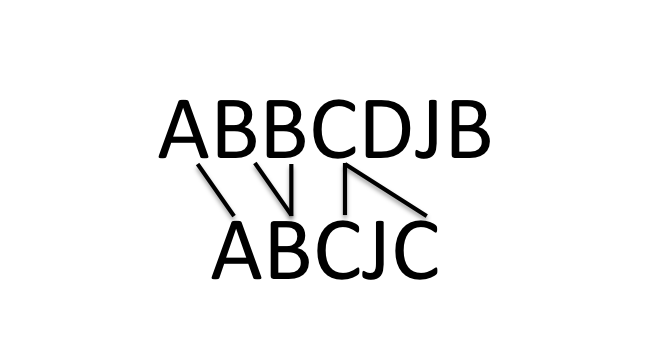
\includegraphics[width=0.25\textwidth]{images/fig2}
			\end{center}
			The runtime of the step where we fill out the grid is on
			the order of $O(n^2)$, as there are only a constant
			number of operations per cell. The backtracking step
			runs on  $O(2n) = O(n)$ because every step we move either up
			or backwards till we get to the top left corner. So the
			total runtime of our algorithm is $O(n^2)$.
			
		\item
			The algorithm I would use here is a modification of the
			Frechet distance algorithm. The key modification I would
			make is not to accept a value $r$ and return
			true if the last two points are under $r$ apart
			and the result of one of the possible sub-problems is
			true.
			Instead return the minimum $r$ 
			for points $P[..i]$ and $Q[..j]$ by returning the maximum of
			the distance between $P[i],Q[j]$ and $k$ where
			$k$ is the minimum of the Frechet distances between:
			\begin{itemize}
			\item $P[..i-1]$ and $Q[..j]$
			\item $P[..i]$ and $Q[..j-1]$
			\item $P[..i-1]$ and $Q[..j-1]$
			\end{itemize}
			Where these vales are calculated in a similar (recursive)
			manner. This will give you the minimum
			Frechet distance as the minimization ensures that you
			pick sequence of moves that results in the lowest 
			Frechet distance. Put another way the minimum Frechet
			distance for $p[..i]Q[..j]$ is either the minimum
			frechet distance between
			$P[..i]$ and $Q[..j-1]$ or
			$P[..i-1]$ and $Q[..j]$ or
			$P[..i-1]$ and $Q[..j-1]$ 
			or the distance between $P[i]$ and $P[j]$ if it's larger
			then the minimum of the three previous quantities. We
			can also use the memoization technique mentioned earlier,
			saving the minimum fringe distance for 
			 $P[..i]Q[..j]$ in cell $i,j$ of our table, starting
			 from the top left corner filling in
			 cells from left to right and rows from top to bottom.
			 At the end of the algorithm report the bottom right
			 cell.\\
			 This algorithm runs on the order of $O(n^2)$ as it
			 requires linear time computation of every cell of an
			 $n$ by $m$ matrix.
		\item 
			To accomplish this, we will fill out a table $F[1..n][1..n]$
		 such that each cell is either blue or
			red. A cell $F[i,j]$ will be blue if the
			distance between $||p_i - q_j|| \leq L$ or red
			otherwise. The desired sequence exists if there is a
			series of either horizontal or vertical steps that get
			you from the top left to the bottom right without
			stepping on a red square. To see why this is, consider
			$F[i][j]$ to represent the points $p_i,q_j$. From
			$p_i,q_j$ the only valid moves are to
			\begin{enumerate}
			\item $p_{i+1},q_{j}$ if $|| p_{i+1} - q_{j}|| \leq L$
			\item $p_{i-1},q_{j}$ if $|| p_{i-1} - q_{j}|| \leq L$
			\item $p_{i},q_{j-1}$ if $|| p_{i} - q_{j-1}|| \leq L$
			\item $p_{i},q_{j+1}$ if $|| p_{i} - q_{j+1}|| \leq L$
			\end{enumerate}
			We can see $p_0,q_0$ is our startpoint and $p_n,q_n$ is
			our endpoint.
			Finding this path will be done with a breadth first
			search from $F[0][0]$ to $F[n][n]$
			marking every node we expanded as expanded and storing
			fringe nodes in a queue \footnote{Because the unweighted edges
			are zero, we don't need to use a priority queue like in
			Dijkstra's algorithm}. If the queue is empty before
			$F[n][n]$ is expanded we know there is no path.\\
			The runtime of the first step is $O(n^2)$ as it requires
			doing one computation for every cell in an $n \times n$
			table.
			The second step runs involves a breadth first search so
			it runs on $O(|V| + |E|)$. Clearly this table has $n^2$
			cells (vertices) and every cell is connected to at most
			$4$ of it's neighbors so the number of edges is at most
			$4n^2$ meaning our algorithm runs on the order of $
			O(4n^2)+ O(n^2) = O(n^2)$.
		\item First construct a table $F[1..n][1..n]$ such that 
				$$F[i][j] = || p_i - p_j ||$$
			then run dijkstra's algorithm from $F[0][0]$ to $F[n][n]$,
			considering every cell connected to (i.e. has edges with) the
			cells directly above, below, and to the right and left
			of it. By the argument in the last question we know that
			these are the only valid moves from any particular
			position. Consider the cost of an
			edge to be the value of the cell it points to. We can
			see that the lowest cost path through the table
			corresponds to the lowest total sum of these lengths,
			and dijkstra's gives us the lowest cost path through
			the table so the solution we find is correct.\\
			The runtime of the first step is still $O(n^2)$ as
			above. However dijkstra's algorithm runs on the order of
			$O(|E|+ |V|\log|V|)$, remembering that $|E| = 4n^2$,
			$|V| = n^2$ the runtime of this phase will be $O(4n^2 +
			n^2 \log{n^2}) = O(4n^2 + 2n^2\log{n}) = O(n^2\log{n})$
\end{enumerate}
\end{document}
